\chapter{Likeness Between Relatives --- Degrees of Relationship}
\label{cha:Lush_Chapter_20}
\index{Relationship|(}

The idea of relationship is familiar to all. Proverbs such as ``Like
father like son,'' ``A chip off the old block,'' ``What's bred in the blood
will out in the bone,'' and ``Blood will tell'' are found in every language.
Their antiquity attests the fact that people have always known
in a general way that offspring tend to resemble their parents, and that
brothers and sisters show many of the same ``family characteristics,''
and that more distant relatives are usually less like each other than close
relatives are. Genetics itself is defined as ``the science which seeks to
account for the resemblances and differences exhibited among organisms
related by descent.''

The first scientific attempts to measure the degrees of resemblance
between different kinds of relatives were made late in the last century
by Sir Francis Galton and his associates. In fact, correlation coefficients
and many of the modern statistical methods now used for other purposes,
too, were devised by them primarily for this purpose. With the
rediscovery of Mendelism, interest in heredity shifted from the biometrical
method to studies of the transmission of individual genes and, for
a time, it was even supposed that the two points of view were antagonistic.
Within recent years many of the statistical consequences of the
Mendelian nature of inheritance have been explored, and the two fields
of knowledge have been unified, each complementing the other.

\section*{THE BASIS OF RELATIONSHIP}
\index{Sampling nature of inheritance|(}

Relatives resemble each other in various degrees because each offspring
gets a sample half of the genes which its parent had. Relationship
between two individuals is simply probability that, because they
are related by descent, they will be alike in more of their genes than
unrelated members of the same population would be. Closer relationship
merely means higher probability of genetic likeness.

The parent-offspring relationship is the simplest one. It is fundamental
in the sense that all other relationships are combinations of
chains of parent-offspring relationships. In populations where there is
no inbreeding, the parent-offspring relationship is 50 per cent, simply
because each offspring has received half of its genes from each parent.
\footnote{Modifications of this for sex-linked genes will be discussed
later in a separate section.} Half of the genes of each offspring are
identical with half of the genes of each parent, since the offspring
received them from that parent. The rest of their genes (those which the
parent did not transmit to this offspring and those which the offspring
received from the other parent) may or may not be alike, just as two
individuals of the same population may have some of the same genes merely
because those genes are common in that population. Where there is some
inbreeding these other genes will have some extra probability of being
alike also. The extra relationship which inbreeding may cause will be
discussed in the next chapter.
\noclub[2]

Half brothers are 25 per cent related because, on the average, one-fourth
of their genes are duplicates which both received from the common
parent, another fourth also came from that parent but are
opposite members of the pair it had, while the remaining half came to
each of them from the parent the other one did not have. This half of
the genes are no more and no less apt to be alike than if the half brothers
were unrelated members of the same population.

The most probable situation among a pair of full brothers is that
one quarter of their genes will be duplicates received from the sire,
another one quarter will be duplicates received from their dam, another
quarter will have come to both from their sire but in each locus the
genes will be opposite members of the pair he had, while the other
fourth will have come to both from their dam but will be opposite
members of the pairs she had.

This fact that pedigree and heredity are not identical was known
before Mendelism but was then regarded as a mystery. Now we know
that it is a natural-indeed an inevitable-consequence of the segregation
of genes in parents which are not completely homozygous. However,
anachronistic traces of the older view still persist in our speech
and writings. Wonder is still sometimes expressed when two brothers
are noticeably unlike, or such unlikeness is inferred to be evidence that
the characteristic in question is not hereditary. In our everyday speech
and among persons unfamiliar with genetics it is not yet generally
appreciated that even for a perfectly hereditary trait (one unaffected by
environment, dominance, or epistasis), full brothers or parent and offspring
will usually differ in half as many of their genes as will unrelated
members of the same population.
\index{Sampling nature of inheritance|)}

The probabilities stated for half and full brothers are averages; that
is, they are more likely to happen than any other one result. Yet the
laws of chance cause some pairs of paternal brothers to receive more
than one quarter of their genes as duplicates from their sire, while other
pairs of brothers get less than one quarter. Although the average or
most probable result remains at one quarter, it is theoretically possible
for paternal brothers to have received anywhere from none to 50 per
cent of their genes as duplicates from their sire. But if the number of
genes is large, either of these extreme happenings would be very rare.
The standard deviation of individual cases around the expected
average of 25 per cent is $25/\sqrt{n}$ per cent where \textit{n} is the
number of independent pairs of genes involved. With $n = 25$, for example, about
two-thirds of all pairs of paternal brothers would have received at
least 20 and not more than 30 per cent of their genes as duplicates from
their sire.\footnote{Linkage makes the \textit{n} of this formula something
more than the number of different linkage groups but less than the total
number of genes involved. With 20 to 30 pairs of chromosomes in most farm
animals, an effective \textit{n} of something like 25 to 100 appears reasonable
for considering the reliability of individual relationship coeffients when
the animals' whole genotypes or their heredity for complicated characteristics
are being considered.} That still leaves room for some individuals actually to be
noticeably more alike in their genes than others which have the same
expected relationship. If we are interested in only one or a very few
pairs of genes, such as the pair for the black-red contrast or the pair for
the horned-polled contrast in cattle, relationship will mean little for a
single pair of animals. However, even for a single pair of genes, the
relationship figure will become dependable if we want to describe the
average situation in a large group of pairs thus related.

\index{Collateral relatives}Each additional generation, which intervenes in the line of descent
through which two individuals are related, halves the fraction of their
genes which are likely to be exact duplicates received from the ancestor
which they have in common. That is why any one line of relationship
between two animals gives an amount of relationship which is \nicefrac{1}{2}
raised to the \textit{n}th power, where \textit{n} is the number of
generations (Mendelian segregations) intervening between the two animals
in that line or path of relationship. If they are related through more
than one line of descent, each such bit of relationship must be evaluated
separately. Then these are added to obtain the total relationship.

Two individuals chosen at random from the population which is
used as the basis for computing the relationship would have many
genes alike, merely because those genes are widespread in that population.
Among pairs of allelic genes chosen at random, $q^2$ will be $AA$ and
$(1 - q)^2$ will be $aa$, leaving only $2q (1 - q)$ of such pairs to be unlike.
Relationship between two individuals is the \textit{extra} likeness due to common
ancestry. It shows what fraction of those genes which would be
unlike in pairs of individuals chosen at random from this same population
are probably alike in the related pair. The average genetic likeness
between random animals of this population is the zero point on the
scale on which relationship is measured. Zero relationship does not
mean absolute unlikeness in every gene any more than zero on the thermometer
needs to mean the coldest temperature possible, or sea level
means the lowest altitude possible.

The question of what population should be used as the base or zero
point for measuring relationship in any particular case thus has some
importance. \index{Evolution}In considering evolutionary questions, the population
might logically be the whole species or even a larger group of some
extremely remote date. This is what the taxonomist means when he
says, for example, that sheep are more closely related to goats than they
are to cattle but are more closely related to cattle than they are to
horses. But in applying the idea of relationship to individual animals
or herds, we never carry it back to such a remote base, partly because
pedigrees necessary for computing relationship are not known that far
back, partly because chance variations from the most probable distribution
of genes will in some cases have been in the same direction in successive
generations and can have become large, and also because the
time involved in evolutionary questions is so enormous that selection
and even mutation have had opportunity to produce important changes
which would not show in the pedigrees. The most remote bases we
actually use in animal husbandry are in connection with the history of
different breeds where we may, for example, group the Jersey and
Guernsey together as ``Channel Island breeds,'' or group together the
black and white lowland cattle of the regions along the shores of the
North and Baltic seas as a group of breeds more closely related to each
other than they are to the Channel Island breeds or to the mountain
breeds of central Europe.

The most convenient population to use for a base in animal breeding
problems with known individual pedigrees is usually the breed at a
date not often more than four to six generations in the past. For example,
two Shorthorns might be ``unrelated'' relative to the Shorthorn
breed in 1910. This is the same thing as saying that they are probably
no more and no less alike genetically than the average pair of Shorthorns
chosen at random from among those born in 1910. Yet, if their
pedigrees were traced further, they might be found to be related 20 per
cent relative to the Shorthorn breed in 1870 and 50 per cent relative to
the foundation animals entered in the very first volumes of the Coates
Herd Book. If their pedigrees could be traced back to the time when
they had ancestors in common with other bovine breeds or races, it
might possibly be found for example, that they are probably alike in 70
per cent of the genes which would be different in random pairs of cattle
from a population which included all cattle now living in Europe.
No practical purpose would be served by tracing pedigrees that far; but
the example may explain the apparent inconsistencies which occur
when we compare relationships between members of the same breed,
between animals of mixed breeding, or between animals belonging to
different breeds or even to different species. The apparent inconsistencies
arise because the populations chosen as bases for computing the
relationships are not the same. The inconsistency is no more a real one
than if we say that a certain mountain peak is 2,500 feet above the plane
at its base but 12,000 feet above sea level. The height of the peak is the
same in either case -- the two figures differ merely because the Lase from
which the height is measured is different in the two cases.

The processes of computing relationship do not allow for changes
which mutation and selection may have caused in gene frequency. The
errors caused by neglecting mutation are not serious unless the base for
relationship was hundreds of generations in the past. Those caused by
neglecting selection might be important for genes with major effects
and under intense selection even when the base date is as recent as six
or eight generations in the past. This is additional reason for not computing
relationships to a distant base date. Instead one considers what
the breed or race average was at a fairly recent date, how it differed
from the average of other breeds, etc., and then considers the two
related individuals in terms of how like each other they probably are in
genes which would have been different in animals descended from the
same breed or race at the base date but without ancestors in common
since.

If two animals are related to an extent which is worth knowing for
practical purposes (i.e., in addition to knowing whether they are members
of the same breed), that relationship will usually come from ancestors
not more than four or five generations back in the pedigrees of
either. Even where there is some reason to express relationship relative
to a more distant base, it is usually sufficient to trace the pedigree to a
date about four or five generations back and then to assume that the
ancestors at that time were a random sample of the breed. For example,
in a study\footnote{Lush, Jay L., Holbert, J. C., and Willham, 0. S. 1936.
Genetic history of the Holstein-Friesian cattle in the United States.
\textit{Jour. of Heredity}, 27:61--72} of Holstein-Friesians born in 1909
these were found to be related to each other about 2.6 per cent relative to
the foundation stock of about 1883. If a present-day Holstein-Friesian is
related 40 per cent to another, both pedigrees being traced back only to
1909, we are not apt to be seriously in error if we assume that the
relationship found if both were traced back to 1883 would be about 41.6 per 
cent (40 per cent plus 2.6 per cent of the remaining 60 per cent). In other
words, 40 per cent relative to 1909 is about the same as 41.6 per cent
relative to 1883 in this breed.

\index{Relationship!measurement of|(}
In human relationships it is usually convenient to assume that the
foundation ancestors in the two pedigrees being compared were random
samples from the same population. This may lead to some discrepancies
in a population like that of the United States, where some
individuals are descended entirely from ancestors coming from one race
while others are descended from crosses between two or more rather distinct
races. People of the same race might consider themselves unrelated
and yet on the average be alike in more of their genes than two first
cousins who come from a racial mixture. If pedigrees were known as far
back as the time when the races originally diverged from each other, the
figures for human relationship would be reasonably consistent also,
except for changes produced by mutation and natural selection and
accumulated chance variations since the races ceased to intermarry
freely. Rut human pedigrees are not known that far. Many people
would have difficulty in even naming all eight of their great grandparents.

\section*{THE MEASUREMENT OF RELATIONSHIP}

Measuring relationship is evaluating the probability that the two
related individuals will have duplicate genes because they are related
by descent. Each line or path of relationship is evaluated separately.
The results are then added to get the total probability of likeness in
their genes. It is oft en convenient to separate direct relationship and
collateral relationship in the computations, although a given percentage
of relationship represents the same probability of genetic likeness,
regardless of whether it is collateral or direct. Direct relationship is that
which comes about because one animal is the ancestor of the other, as
parent and offspring or grandsire and grandson. Collateral relationship
is that which comes about because both animals are descended in part
from some of the same ancestors, as half and full brothers, uncle and
niece, cousins, etc.

The first thing to do is to examine the pedigrees and find all the
paths or lines of descent by which the two animals are related. To evaluate
the closest paths first is usually more convenient and less likely to
lead to duplication or omissions. Usually two individuals are not connected
by many different paths of relationship unless there has been
some inbreeding.

Direct relationship is measured by what animal breeders commonly
call ``percentage of blood.'' By ``blood'' is meant inheritance in general
or the genes considered collectively. The physical substance, blood, is
not actually transmitted from parent to offspring at all. The young
embryo makes its own blood. Figure~\ref{fig:Lush_Figure_29} shows the percentages of
``blood'' arranged in the form of a pedigree. The fractions come naturally
out of the halving nature of Mendelian segregation.

\begin{figure}
	\centering
    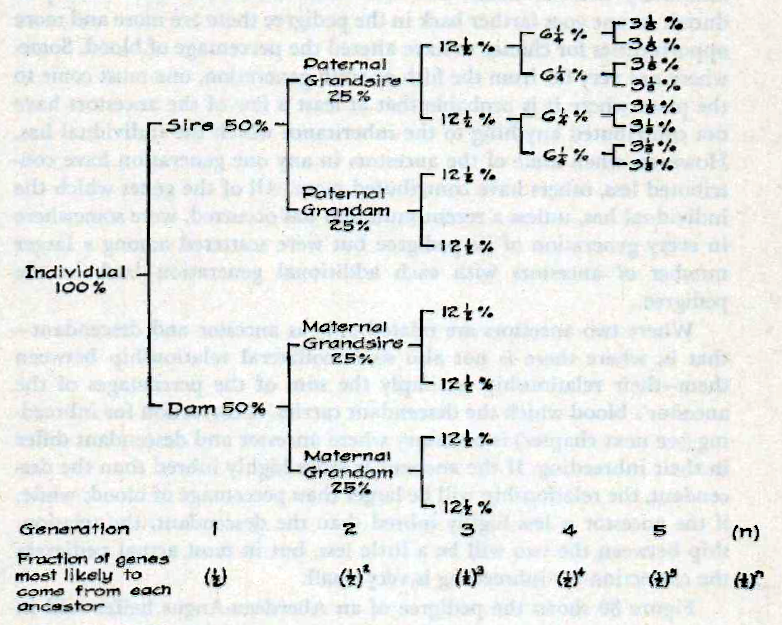
\includegraphics[width=\textwidth]{Figure_29.png}
    \caption{The fraction of an individual's genes most likely to come from each ancestor.}
    \label{fig:Lush_Figure_29}
\end{figure}

\index{Percentage of blood|(}
The most probable proportion of an individual's genes to come
from each of its ancestors is 50 per cent from a parent, 25 per cent from
a grandparent, 12\nicefrac{1}{2} per cent from a great grandparent, and so on, the
percentage being halved with each additional generation the ancestor
is farther back in the pedigree. Because of the part chance plays in
Mendelian inheritance, these percentages need not be exact for an
ancestor farther back than a parent. So far as concerns any one great,
great, great grandparent, the most probable expectation is that the individual
will have inherited \nicefrac{1}{32} of all its genes from that ancestor. Even
in animals having 30 pairs of \index{Chromosomes}chromosomes, this does not average quite
two chromosomes from each ancestor in that generation. Since there is
some crossing-over, it is probable that the individual will still have at
least a few genes from every ancestor in that generation. However, it
could happen that certain ancestors in that generation would have contributed
nothing at all to this individual's inheritance. So far as concerns
the inheritance which the descendant has, such ancestors might as
well never have existed except that they were a part of the living
machinery without which this individual would not have been produced.
As one goes farther back in the pedigree there are more and more
opportunities for chance to have altered the percentage of blood. Somewhere
not very far from the fifth or sixth generation, one must come to
the place where it is probable that at least a few of the ancestors have
not contributed anything to the inheritance which the individual has.
However, when some of the ancestors in any one generation have contributed
less, others have contributed more. All of the genes which the
individual has, unless a recent mutation has occurred, were somewhere
in every generation of its pedigree but were scattered among a larger
number of ancestors with each additional generation back in the
pedigree.

Where two ancestors are related only as ancestor and descendant that
is, where there is not also some collateral relationship between
them -- their relationship is simply the sum of the percentages of the
ancestor's blood which the descendant carries. A correction for inbreeding
(see next chapter) is necessary where ancestor and descendant differ
in their inbreeding. If the ancestor is more highly inbred than the descendant,
the relationship will be larger than percentage of blood; while,
if the ancestor is less highly inbred than the descendant, the relationship
between the two will be a little less, but in most actual pedigrees
the correction for inbreeding is very small.

Figure~\ref{fig:Lush_Figure_30} shows the pedigree of an Aberdeen-Angus heifer sold in
1931 in the Strathmore sale. This heifer ``carries 81\nicefrac{1}{4} per cent of the
blood of'' Earl Marshall. This figure is the sum of: 25 per cent for each
of Earl Marshall's two appearances as grandsire, 12\nicefrac{1}{2} per cent for each
of his two appearances as great grandsire, and 6\nicefrac{1}{4} per cent for his one
appearance as great great grandsire in this pedigree. By similar computations
it will be seen that Earl Marshall 50th carries 87\nicefrac{1}{2} per cent of
the blood of Earl Marshall and that Blackcap Empress 74th carries 75
per cent of the blood of Earl Marshall. The percentage of Earl Marshall
blood in the daughter is naturally the average of that in her parents.
These figures for percentage of blood need only a small correction for
inbreeding (larger than usual in this case) to become the coefficients of
relationship of Earl Marshall to these three descendants of his.

\index{Collateral relatives|(}Collateral relationship between two animals is computed separately
for each line of descent by which it is possible to go from one of them
back to the common ancestor and then down to the other. Each generation
in this line of descent is another Mendelian segregation halving the
fraction of genes which are likely to be duplicates in the two animals
because of their common descent. If there are many more than four or
five intervening segregations, the amount of relationship through any
one such line will be insignificantly small; but if there are many such
lines, their total may be large enough to be of some importance.
\noclub[2]

\begin{figure}
	\centering
    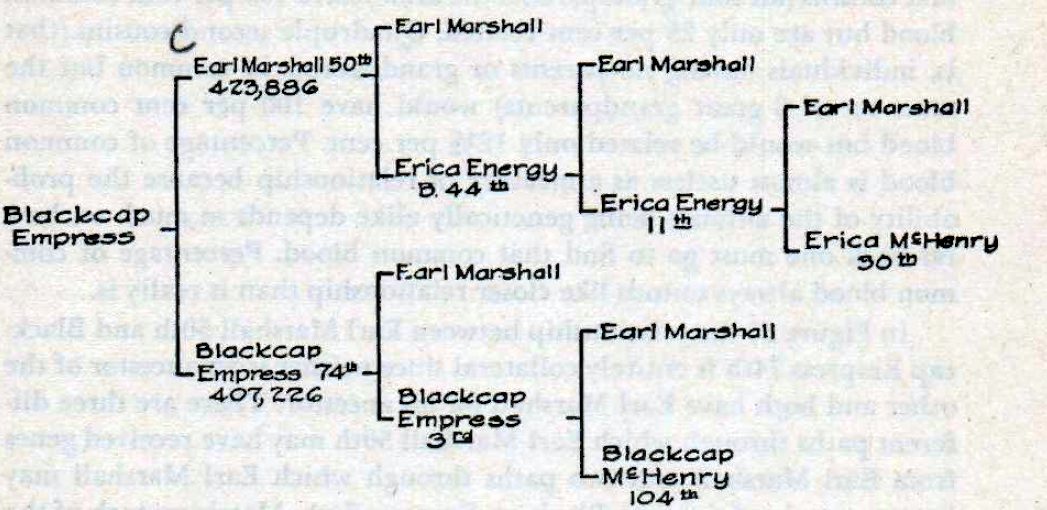
\includegraphics[width=\textwidth]{Figure_30.png}
    \caption{A pedigree showing high relationship to the Aberdeen-Angus bull, Earl
			 Marshall.}
    \label{fig:Lush_Figure_30}
\end{figure}

The probability that cousins will have the same genes may be computed
by extending the same process used for computing the relationship
between half brothers. For each pair of genes the chance is one-half
that a grandparent will give the same gene to both its offspring. Only
one-half the times when this does happen will this same gene be transmitted
to the one cousin. In only one-half of those cases will the other
offspring transmit the same gene to the other cousin. There is, therefore,
one chance in eight that an identical gene shall reach two cousins
from a common grandparent. Even this concerns only half of their
inheritance, since the other half comes from their other parent. Hence
the probable genetic likeness between cousins on account of common
descent from one grandparent is that \nicefrac{1}{16} of their genes will be identical
because of this. If, as is usually the case with human first cousins,
they have two grandparents in common, this adds an equal probability
of their having the same genes through descent from that other grandparent.
This makes a total probability that \nicefrac{1}{8} of their genes will be
alike because of the common ancestry, while the rest of their genes are
no more and no less apt to be alike than if they were unrelated members
of the same freely interbreeding population.

Breeders sometimes measure collateral relationship by ``percentage
of common blood,'' but this can be very misleading. Full brothers have
100 per cent common blood but are only 50 per cent related; double
first cousins (all four grandparents the same) have 100 per cent common
blood but are only 25 per cent related. Quadruple second cousins (that
is, individuals having no parents or grandparents in common but the
same set of 8 great grandparents) would have 100 per cent common
blood but would be related only 12\nicefrac{1}{2} per cent. Percentage of common
blood is almost useless as a measure of relationship because the probability
of the animals being genetically alike depends so much on how
far back one must go to find that common blood. Percentage of common
blood always sounds like closer relationship than it really is.

In Figure~\ref{fig:Lush_Figure_30} the relationship between Earl Marshall 50th and Blackcap
Empress 74th is entirely collateral since neither is an ancestor of the
other and both have Earl Marshall for an ancestor. There are three different
paths through which Earl Marshall 50th may have received genes
from Earl Marshall and two paths through which Earl Marshall may
have transmitted genes to Blackcap Empress 74th. Matching each of the
three ways with each of the two ways makes six different ways in which
these two descendants of Earl Marshall might have received duplicates
of any gene which was in him. The fact that Earl Marshall is the
sire of both contributes 25 per cent to their relationship. The two different
ways in which he is the sire of one and the grandsire of the other
contribute 12\nicefrac{1}{2} per cent each. Descent from him as grandsire on both
sides contributes 6\nicefrac{1}{4} per cent. Descent from him as sire of one and great
grandsire of the other contributes another 6\nicefrac{1}{4} per cent. Finally the
small probability that these two animals would get identical genes by
the long route from Earl Marshall as great grandsire of one and grandsire
of the other contributes another 3\nicefrac{1}{8}  per cent to their relationship.
This makes a total of 65\nicefrac{51}{8} per cent, all of it coming through their descent
from Earl Marshall, but that is still to be corrected for their
inbreeding. A somewhat simpler way of figuring their relationship in
this case, where they have only one ancestor in common, is to find that
one of them has 75 per cent of the blood of Earl Marshall, while the
other has 87\nicefrac{1}{2} per cent, and to \textit{multiply} those two percentages together.
This method gives the same answer; but if the two animals had more
than one ancestor in common, the computations would have to be made
separately for each such ancestor. This method will lead to difficulties
if the common ancestors are related to each other.

These rules for computing relationships are nothing but counting
the number of Mendelian segregations which have intervened in each
line of descent connecting two individuals, and using $(1/2)^n$ aas the fraction
of their genes which are likely to be identical because the two animals
received duplicate genes in that way from their common ancestor.

When one animal is an ancestor of the other and they are also
related collaterally because both are descended from a third animal, it
is usually more convenient to compute the direct relationship first. An
example of this can be had from Figure~\ref{fig:Lush_Figure_30} if we wish to learn how closely
Earl Marshall 50th is related to his daughter, Blackcap Empress.
They are directly related as sire and daughter, and in addition he may
have received from Earl Marshall some genes for which she received
duplicates through her dam. He traces to Earl Marshall in three different
lines, the number of generations in each being 1, 2, 3, respectively,
while she traces through her dam to Earl Marshall in two lines, the
number of generations being 2 and 3 in those. Combination of each of
the two with each of the three makes six different ways in which these
two animals may have received duplicate genes by descent from Earl
Marshall. The sum of the separate values for these six paths equals
32 \nicefrac{13}{16} per cent collateral relationship to be added to the 50 per cent
direct relationship. That total is still to be corrected for the inbreeding,
which in this case is intense enough to make that correction rather
large.

Figure~\ref{fig:Lush_Figure_31} shows another example. The relationship of X to A is
both direct and collateral, while the relationship between X and Z is
entirely collateral, neither being an ancestor of the other. The arrow
diagram of the pedigree is often very convenient for showing at a glance
the nature of the relationship. If the pedigrees are complicated by much
inbreeding, the arrow diagram is almost necessary in order not to omit
some lines of relationship nor count some a second time without being
aware of having done so. The relationship of X to Z in Figure~\ref{fig:Lush_Figure_31} will
illustrate why percentage of common blood is not dependable as a
measure of collateral relationship. It is not legitimate to say that 75 per
cent of X's blood is the same as 100 per cent of Z's blood and to estimate
their relationship through manipulating these figures of ``common
blood'' in any way. It is legitimate to do this separately for each common
ancestor and to say that Z has 50 per cent of the blood of D and X
has 25 per cent of that blood and that Z and X are therefore related 50
per cent of 25 per cent, or 12½ per cent, through D. Also, it is legitimate
to say that both Z and X have 50 per cent of the blood of C and
that 50 per cent of 50 per cent equals 25 per cent of relationship
between Z and X through descent from C. This 25 per cent may then
be added to the 12\nicefrac{1}{2} per cent of relationship through D to give the total
relationship of 37\nicefrac{1}{2} per cent.
\index{Collateral relatives|)}
\index{Percentage of blood|)}

Relationship between two individuals cannot be higher than 50 per
cent unless some inbreeding has been practiced. The only exception to
this concerns identical twins, and members of the same ``clone'' in
plants and animals which can be propagated asexually. Relationship
between members of such isogenic lines is 100 per cent, since they are
really duplicates of the same zygote and there has been no intervening
Mendelian segregation or recombination to permit them to have unlike
genes. Since not much inbreeding occurs in most animal species or in
man, we rarely have a chance to see the resemblance between animals
related much more closely than 50 per cent. It is largely for this reason
that identical twins\index{Identical twins} are such interesting evidence about the importance
of heredity. An increase from 50 to 100 per cent in genetic likeness
makes a marked difference in the variation to be expected between individuals,
especially in characteristics which are highly hereditary.

\begin{figure}
	\centering
    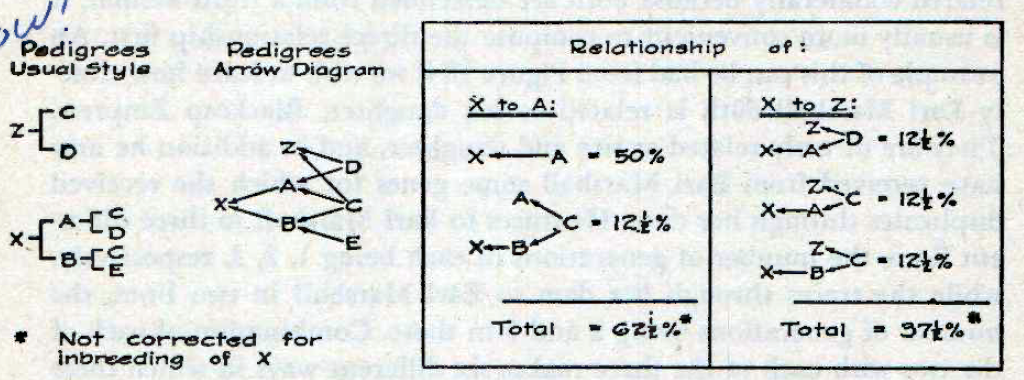
\includegraphics[width=\textwidth]{Figure_31.png}
    \caption{Showing how relationship is computed.}
    \label{fig:Lush_Figure_31}
\end{figure}

Two animals cannot be very closely related if all their common
ancestors are distant ones. Rarely is much gained by going back farther
than three or four generations in the pedigrees of two animals to see
whether they are related. In an extreme case two animals might have
the very same 16 great great grandparents, and yet their relationship to
each other would be only 6\nicefrac{1}{4} per cent if they had no parents, grandparents,
or great grandparents in common and if there were no inbreeding
involved.

Relationship is sometimes measured in ``degrees,'' especially for
legal purposes. In civil law a degree of relationship corresponds to a
generation of Mendelian segregation. Thus parent and offspring are
``related in the first degree,'' grandparent and offspring are ``related in
the second degree,'' uncle and nephew are ``related in the third degree,''
etc. When the individuals are related through more than one line of
descent, each line is computed and stated separately without combination
into a single figure. In canon law and common law only the number
of generations in the longer line of descent from the common
ancestor is counted. Thus uncle and nephew are related in the second
degree by canon law and common law.

\section*{THE EFFECTS OF SEX-LINKAGE}
\label{page255}
\index{Sex linkage}

In the mammals the male is the heterogametic sex. His sex-linked
inheritance comes entirely from his mother. Her sex-linked inheritance
is present in duplicate, and among the pairs of sex-linked genes which
are heterozygous in her, chance at segregation determines what sex-linked
inheritance a son shall receive. The result is that 100 per cent of
his sex-linked genes are like 50 per cent of hers. The square root of the
product of these is the relationship (71 per cent) of son and dam for sexlinked
genes. The sex-linked inheritance of a female comes equally
from both parents; but since her sire does not have a duplicate set of
sex-linked genes, chance plays no part in determining what sex-linked
inheritance she shall receive from him. So far as his daughters are concerned,
the situation is the same as if the sire were homozygous for all
his sex-linked genes. The relationship between sire and daughter is also
71 per cent for sex-linked genes, since 100 per cent of those in the sire
are like 50 per cent of those in his daughter. Daughter and dam are
related 50 per cent for sex-linked genes, just as they are for autosomal
genes. Sire and son are not related at all for sex-linked genes, since the
son cannot receive any of those from his sire. The practical consequence
of sex-linkage is to make the parent-offspring relationship higher
between opposite sexes than it is between parent and offspring of the
same sex. In birds, moths, and some fishes the female is heterogametic,
but that leaves the practical situation nearly the same: namely, that
males are a bit more closely related to their dams and females to their
sires than either is to the parent which is the same sex. The lowest relationship
for sex-linked genes is that between sire and son in the mammals,
but between dam and daughter in birds.

This difference in relationship to ancestors of different sexes is
partially, but not entirely, equalized as one goes further back in the
pedigree , since a dam may transmit either the sex-linked genes she got
from her sire or the sex-linked genes she got from her dam.

Since the farm animals have about 20 to 30 pairs of \index{Chromosomes}chromosomes
and only one pair carries the sex-linked genes, it is improbable that the
total amount of sex-linked inheritance is much larger than 3 to 5 per
cent of the total inheritance. Hence, for practical purposes no material
error is introduced by neglecting sex-linkage when computing relationships.
(See table \ref{tbl:Lush_Table_20}.) Occasionally there may be individual matings in
which sex-linkage will play a noticeable part.
\index{Relationship!measurement of|)}

\section*{PRACTICAL USES OF THE RELATIONSHIP COEFFICIENT}
\index{Ancestors, importance of various ones|(}
\index{Pedigrees as aids to selection|(}

The most important practical use of the relationship coefficient is to
predict the merit of relatives of animals whose merit is known. This is
the whole basis for using the merit of relatives to aid in making selection
more effective. If nothing at all is known about an animal or its
relatives, the only prediction we can make is that it will be an average
animal of its breed. Neglecting for the moment the effects of environment,
dominance, epistasis, and selection, if we know an animal related
40 per cent to the unknown one, the most probable prediction is that
the unknown animal will deviate from the breed average in the same
direction as the known relative does, but only 40 per cent as far. If a
cow's genotype for fat production is 100 pounds above the breed average
the most probable genotype of her daughter, if nothing is known
about the sire except that he belonged to the same breed, is that the
daughter's genotype will be 50 pounds above the breed average.
Numerous practical difficulties and necessary precautions beset this use
of relationship as a measure of how much weight to put on each relative
in estimating the breeding worth of an animal. Most of those hinge
around the inescapable fact that we are not sure of the genotypes of the
relatives but only know their apparent merit. The two may be widely
different if outward merit is much affected by environment, dominance,
or epistasis. Other difficulties concern the weight to give each relative in
combining information about several related ones, not all known equally
well, into the best single estimate of what the unknown animal will
be. The practical aspects of this were discussed in chapter \ref{cha:Lush_Chapter_14}. They put
serious limitations on the practical usefulness of the principle-which is
true when comparing equally well-known relatives of which one is to
be used alone in such estimates-that the attention to be given such
relatives is in proportion to their relationship to the animal to be estimated.
The relationship between an individual and the average genotype
of a group of its relatives may be higher than its relationship to
any one of them. The simplest and most important example of this is
the case of half sibs. In the extreme case of a characteristic perfectly
hereditary in the simple additive way, and unselected half sibs from a
random breeding population, the equation for predicting with the
least error what an individual will be from knowing \textit{p} of its paternal
half sibs and \textit{m} of its maternal half sibs is:

{\setlength{\tabcolsep}{0.1em} % for the horizontal padding}
\begin{table}[h]
	\centering
	\begin{tabular}{lll}
		Animal $=$ breed average & \(+ \dfrac{p}{p + 3}\) & (paternal half sibs minus breed\\
			   					 & 						  & average)\\
			   					 & \(+ \dfrac{m}{m + 3}\) & (maternal half sibs minus breed\\
			   					 & 						  & average)\\
	\end{tabular}
\end{table}

\noindent
As \textit{p} and \textit{m} increase from one to at least four or five, the usefulness of
this equation goes up rapidly and it soon comes close to the limit set by
perfect knowledge of the genotypes of sire and dam of the individual
being predicted. Of course, in actual practice there are effects of environment
and dominance and \index{Epistatic effects}epistasis and possible previous selection of
half sibs which will usually make it wise to put less weight than this on
what the half sibs indicate. The above equation shows quantitatively
what we are recommending if we advise choosing a son of a proved sire
and a proved dam.

To the extent that the trait being measured is affected by environment,
dominance, and epistasis, actually observed likeness will be less
than the genetic likeness unless each pair of related individuals tended
to be exposed to an environment alike for them but different from the
environment of other pairs. In that case the observed may be higher
than the calculated. Thus, in a random bred population hal£ sisters are
genetically as much alike as grandam and granddaughter; but each pair
of half sisters is more apt to have been exposed to the same more or less
unusual environment than is each grandam and granddaughter pair.
Hence, in such data as official dairy records, it is to be expected that the
observed likeness between half sisters will be larger than that between
grandam and granddaughter. For the same reason paternal half sisters,
which are usually contemporaries, may be expected actually to resemble
each other a little more closely than maternal half sisters. The latter
may have been born and reared several years apart.

\index{Dominance}Dominance and epistasis make observed likenesses generally lower
than calculated ones, but in certain relationships-of which the most
important is that between full sibs-dominance produces a little extra
likeness on its own account. This partly offsets its general tendency to
lower likenesses.

If breeders' ideals diverge enough that they have been selecting for
distinctly different types within the same breed, then animals in the
same herd are apt to resemble each other, relative to the whole breed,
more than their relationships indicate.
\index{Ancestors, importance of various ones|)}
\index{Pedigrees as aids to selection|)}
\noclub[3]

\section*{GALTON'S LAW}
\index{Galton's ``Law''|(}

Two distinct although related ideas are sometimes confused under
the name ``Gallon's Law.'' The first is the observed fact that the correlation
between parent and offspring is nearly $+ .50$ in populations
where there is not much inbreeding and where the trait being measured
is highly hereditary. The correlation between an animal and a more
remote ancestor is halved for each additional generation which separates
them. This is precisely what was shown in Figure~\ref{fig:Lush_Figure_29} and was
discussed under ``percentage of blood.''\index{Percentage of blood} It was an observed fact in Galton's
time and had been used by practical breeders in England from at least
as long ago as 1815.\footnote{According to the encyclopedia of J. G. Krtinitz}
The only material difference now is that we understand
why it is a natural consequence of the laws of inheritance, provided
the population is mating at random and the trait being studied is
entirely hereditary in the simple additive manner. Naturally the extent
to which these conditions are fulfilled varies in different populations
and even for different traits in the same population and often is known
only within rather wide limits.

\begin{figure}[!htbp]
	\centering
    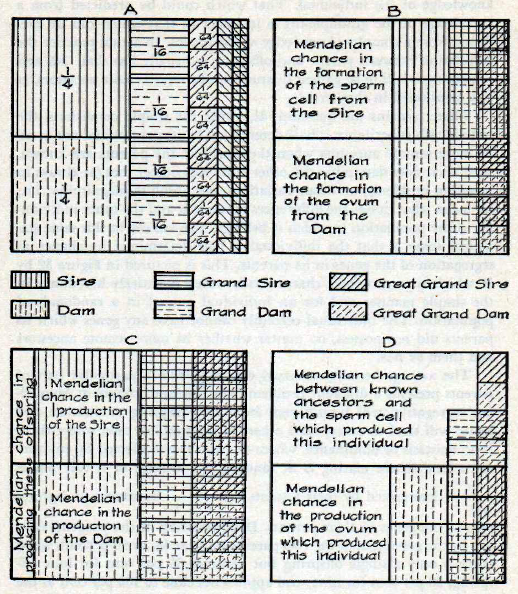
\includegraphics[width=.9\textwidth]{Figure_32.png}
    \caption{Galton's ``law'' of the relative importance of various ancestors, pictured
			 for a characteristic perfectly hereditary in the simple additive way. A: As formulated
			 by Galton, each ancestor being considered singly. B: Correctly pictured for an individual
			 animal in a random breeding population. That which can be predicted from
			 the more remote ancestors is included in what can be predicted from the intervening
			 ancestors. Mendelian chance at segregation accounts for half of the determination in
			 the statistical sense of that word. C: Same as B except that this concerns the average
			 inheritance of nine unselected offspring from one pair of parents. The effects of
			 chance in the nine segregations which produced the sperm cells and in the nine 
			 segregations which produced the ova tend Lo cancel each other to such an extent that
			 Mendelian chance now determines only one-tenth of the average inheritance of these
			 nine instead of the one-half which it determines for each individual. D: Determination
			 of the individual by known characteristics of its ancestors in the case where
			 males cannot express the characteristic themselves and neither the sire nor the two
			 grandsires were progeny-tested.}
    \label{fig:Lush_Figure_32}
\end{figure}

The other part of Galton's law --- which unfortunately is the part
most frequently quoted --- is true only in a specialized statistical sense.
The square of the correlation coefficient measures the portion of the
variance in one variable which disappears in data in which the other
variable is constant. In this special statistical sense the individual's
inheritance is \nicefrac{1}{4} determined by its sire and¼ by its dam. That instantly
raises the question: What determines the remaining \nicefrac{1}{2}? Galton reasoned
that this same process would be repeated with the sire and with
the dam, each of them being \nicefrac{1}{4} determined by its sire and another \nicefrac{1}{4}
by its dam, and that if this process were pursued far enough the fractions
would ultimately add up to one. Consequently he proposed as a
general ``law'' that the individual's inheritance was \nicefrac{1}{4} determined by
its sire and \nicefrac{1}{4} by its dam, \nicefrac{1}{16} by each of the
four grandparents, \nicefrac{1}{64} by each of the 8 great grandparents, and
so on, each ancestor contributing just \nicefrac{1}{4} as much to the total
inheritance as did the one a generation nearer to the individual. This is
usually pictured as in A, of Figure~\ref{fig:Lush_Figure_32}. Because this
seemed a logical scheme, it was accepted rather widely
and even today is sometimes quoted with approval. Unfortunately, the
obvious inference from this diagram (that if one knew all about all of
the ancestors, he would know all about the heredity of this individual)
is not true.

\begin{figure}[!htbp]
	\centering
    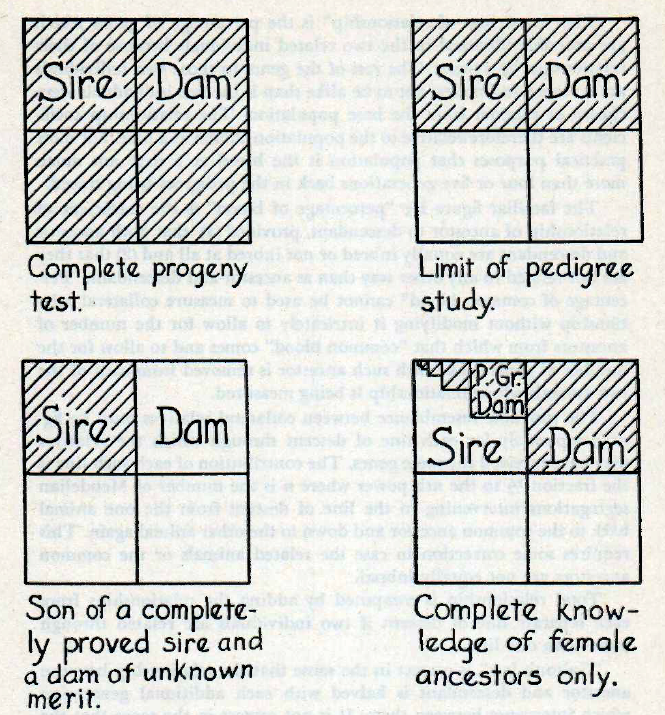
\includegraphics[width=.9\textwidth]{Figure_33.png}
    \caption{Relative accuracy of a progeny test and of various kinds of pedigrees
			 when the information in each is as complete as is theoretically possible under the
			 conditions named. Shaded areas represent portions of the individual's inheritance
			 determined (in the statistical sense) by complete information of the kind pictured.
			 The correlation between the acmal and the predicted breeding value of the indi vidual
			 would be the square root of the shaded fraction of the area; i.e., 1.0 in the
			 upper lefthand corner, .71 in the upper right, .50 in the lower left, and .58 in the
			 lower right. The unshaded areas represent possibilities for Mendelian segregation to
			 have made the individual's actual breeding value higher or lower than its expected
			 breeding value.}
    \label{fig:Lush_Figure_33}
\end{figure}

Had Galton used multiple correlation technique (as Yule pointed
out at the third International Genetics Congress in 1906) he would
have found that the partial correlation between grandparent and
grandson or granddaughter, the intervening parent being held constant,
is zero in any population in which the correlation between parent
and offspring is .50 and the correlation between grandparent and
grandson or granddaughter is .25. If the parent's heredity is not known,
it is still true in the technical statistical sense of the word that the individual
is ``determined'' \nicefrac{1}{16} by each of its grandparents. That is shown
for the paternal grandam by D in Figure~\ref{fig:Lush_Figure_32}. But if the parent's heredity
is known, knowledge of the grandparents adds nothing to the
knowledge of the individual. That which could be predicted from a
knowledge of the grandparent is included in that which can be pre- ·
dieted from a complete knowledge of the parent. In actual practice the
correlation between parent and offspring is usually less than .50, and
something is still to be gained by studying the more remote ancestors, as
was mentioned in chapter~\ref{cha:Lush_Chapter_14}.

There remains the question: If, under the simple conditions, the
individual's inheritance is half determined by its parents and not at all
by more remote ancestors when the merits of the parents are known,
then what does determine the other half? Remember that (as always in
breeding problems) we mean variations, not absolute magnitudes; i.e.,
we mean what causes the differences between it and the other individuals
in the population to which it belongs. The answer in this same statistical
sense is that the individual is half determined by chance at
segregation of the genes in its parents. This is pictured in
Figure~\ref{fig:Lush_Figure_32} by B, which is correct for a characteristic
which is entirely hereditary in the simple manner and for an individual
animal in a random-bred population. The individual certainly cannot have
any genes which its parents did not possess, no matter whether its more
remote ancestors had them or not.

\index{Progeny test|(}
The average heredity of many offspring from a particular pair of
parents presents a different problem. The results of chance at Mendelian
segregation will be different from one offspring to another and
hence will tend to cancel each other. In the simplest case, where there
is no epistasis or dominance, where the trait is not affected by environment,
and where mating is at random, the average of \textit{n} full sibs is
$\dfrac{n}{n + 1}$ determined by their parents and $\dfrac{1}{n + 1}$ by chance at
segregation of the genes in their parents. Determination of the progeny average
by the genotypes of the two parents starts at \nicefrac{1}{2}, or 50 percent, when
there is only a single offspring but becomes 80 per cent for four offspring,
90 per cent for nine, and approaches close to 100 per cent as the
numbers of offspring become very large. This is pictured in C of
Figure~\ref{fig:Lush_Figure_32} for the case where \textit{n} = 9. This is why complete knowledge of 
the genotypes of the parents would permit predicting with almost perfect
accuracy what the average of their progeny (if numerous) will be, even
though it would not permit highly accurate prediction of what each
individual offspring will be. D of Figure~\ref{fig:Lush_Figure_32} shows Galton's law when
the merits of some of the near ancestors on one side of the pedigree are
not known.
\index{Galton's ``Law''|)}
\index{Progeny test|)}

\section*{SUMMARY}

The genetic resemblance between individuals is based on the probability
that they have received identical genes from animals which are
ancestors of them both.

The ``coefficient of relationship''	 is the percentage of genes which
are probably identical in the two related individuals because of their
relationship by descent. The rest of the genes in those two individuals
are no more and no less apt to be alike than if the two individuals were
chosen at random from the base population. The relationship coefficients
are therefore relative to the population chosen as a base. For most
practical purposes that population is the breed at a date not much
more than four or five generations back in the pedigrees being traced.

The familiar figure for ``percentage of blood''\index{Percentage of blood} is the coefficient of
relationship of ancestor to descendant, provided (l) that both ancestor
and descendant are equally inbred or not inbred at all and (2) that they
are not related in any other way than as ancestor and descendant. ``Percentage
of common blood'' cannot be used to measure collateral relationship
without modifying it intricately to allow for the number of
ancestors from which that ``common blood'' comes and to allow for the
number of generations each such ancestor is removed from each of the
two animals whose relationship is being measured.

The probable resemblance between collateral relatives must be figured
separately for each line of descent through which the relatives
may have received the same genes. The contribution of each such line is
the fraction \nicefrac{1}{2} to the \textit{n}th power where \textit{n}
is the number of Mendelian segregations intervening in the line of descent
from the one animal back to the common ancestor and down to the other
animal again. This requires some correction in case the related animals
or the common ancestors are not equally inbred.

Total relationship is computed by adding the relationships from
each separate line of descent if two individuals are related through
more than one line.

``Gallon's law'' is correct in the sense that the relationship between
ancestor and descendant is halved with each additional generation
which intervenes between them. It is not correct in the sense that the
individual's heredity is completely determined by the heredity of its
ancestors. In that sense in a random-bred population the individual is
one-fourth determined by each parent and one-half determined by
chance in Mendelian segregation. Determination by more remote ancestors
is included in the determination by the parent.

The existence of sex-linkage causes sons to resemble dams a little
more than they do their sires and makes daughters resemble their sires
a bit more closely than they do their dams. This effect must be small in
most cases.

Relationship measures the probability that individuals will be alike
\textit{in their genes}. Their actual outward likeness depends also upon how
much the traits being measured are affected by environment, dominance,
and epistasis, upon the extent to which their environments were
correlated, and upon whether their ancestors were mated like to like.

The most important practical use for relationships is in predicting
the most probable merit of unknown or perhaps even unborn individuals
from the merit of their known relatives.

\section*{REFERENCES}

\begin{hangparas}{0.5in}{1}%
Davenport, E. D. 1907. Principles of breeding, pp. 525--34.

Fairchild, David . 1921. A genetic portrait chart. Jour. of Heredity, 12:213--19.

Wright, Sewall. 1922. Coefficients of inbreeding and relationship. Amer. Nat., 56:330--38.

---. 1923. Mendelian analysis of the pure breeds of livestock. I. The measurement
of inbreeding and relationship. Jour. of Heredity, 14:339--48.
\end{hangparas}
\index{Relationship|)}